\section{Experiments \& Results}

% We implement TC $G$-Pooling for the groups $SO(2)$ (discretized as $C_n$), and $O(2)$ (discretized as $D_n$) acting on $\mathbb{R}^2$ and the groups $SO(3)$ (discretized as the Chiral Octahedral group $O$) and $O(3)$ (discretized as the Full Octahedral group $O_h$) acting on $\mathbb{R}^3$.

\subsubsection*{Implementation}

We implement the $G$-TC Layer for arbitrary discretized groups with an efficient implementation built on top of the \href{https://github.com/QUVA-Lab/escnn}{ESCNN library} \cite{cesa2022a, e2cnn}, which provides a general implementation of $E(n)$-Equivariant Steerable Convolutional Layers. The method is flexibly defined, requiring the user only to provide a (Cayley) table that defines the group's product structure. The code is publicly available at \url{https://github.com/sophiaas/gtc-invariance}. Here, we demonstrate the approach on the groups $SO(2)$, and $O(2)$, $SO(3)$, and $O(3)$, discretized as the groups $C_n$ (cyclic), $D_n$ (dihedral), $O$ (chiral octahedral), and $O_h$ (full octahedral), respectively. \href{https://github.com/QUVA-Lab/escnn}{ESCNN} provides implementations for $G$-Conv layers on all of these $E(n)$ subgroups.

% For all experiments, we make use of the \href{https://github.com/QUVA-Lab/escnn}{ESCNN library} \cite{cesa2022a, e2cnn}, which provides a general implementation of $E(n)$-Equivariant Steerable Convolutional Layers, including layers equivariant to the subgroups of $E(n)$ we consider here. [Insert computational strategy and reference algorithm in appendix.]


\subsubsection*{Experimental Design}

We examine the performance of the $G$-TC over Max $G$-Pooling in $G$-Equivariant Networks defined on these groups and trained on $G$-Invariant classification tasks. For the groups $SO(2)$ and $O(2)$ acting on $\mathbb{R}^2$, we use the MNIST dataset of handwritten characters \cite{lecun1998mnist}, and for the groups $SO(3)$ and $O(3)$ acting on $\mathbb{R}^3$, we use the voxelized ModelNet10 database of 3D objects \cite{wu20153d}. We generate $G$-MNIST and $G$-ModelNet10 datasets by transforming the domain of each signal in the dataset by a randomly sampled group element $g \in G$ (Figure \ref{fig:datasets}).


\begin{figure}
    \centering
    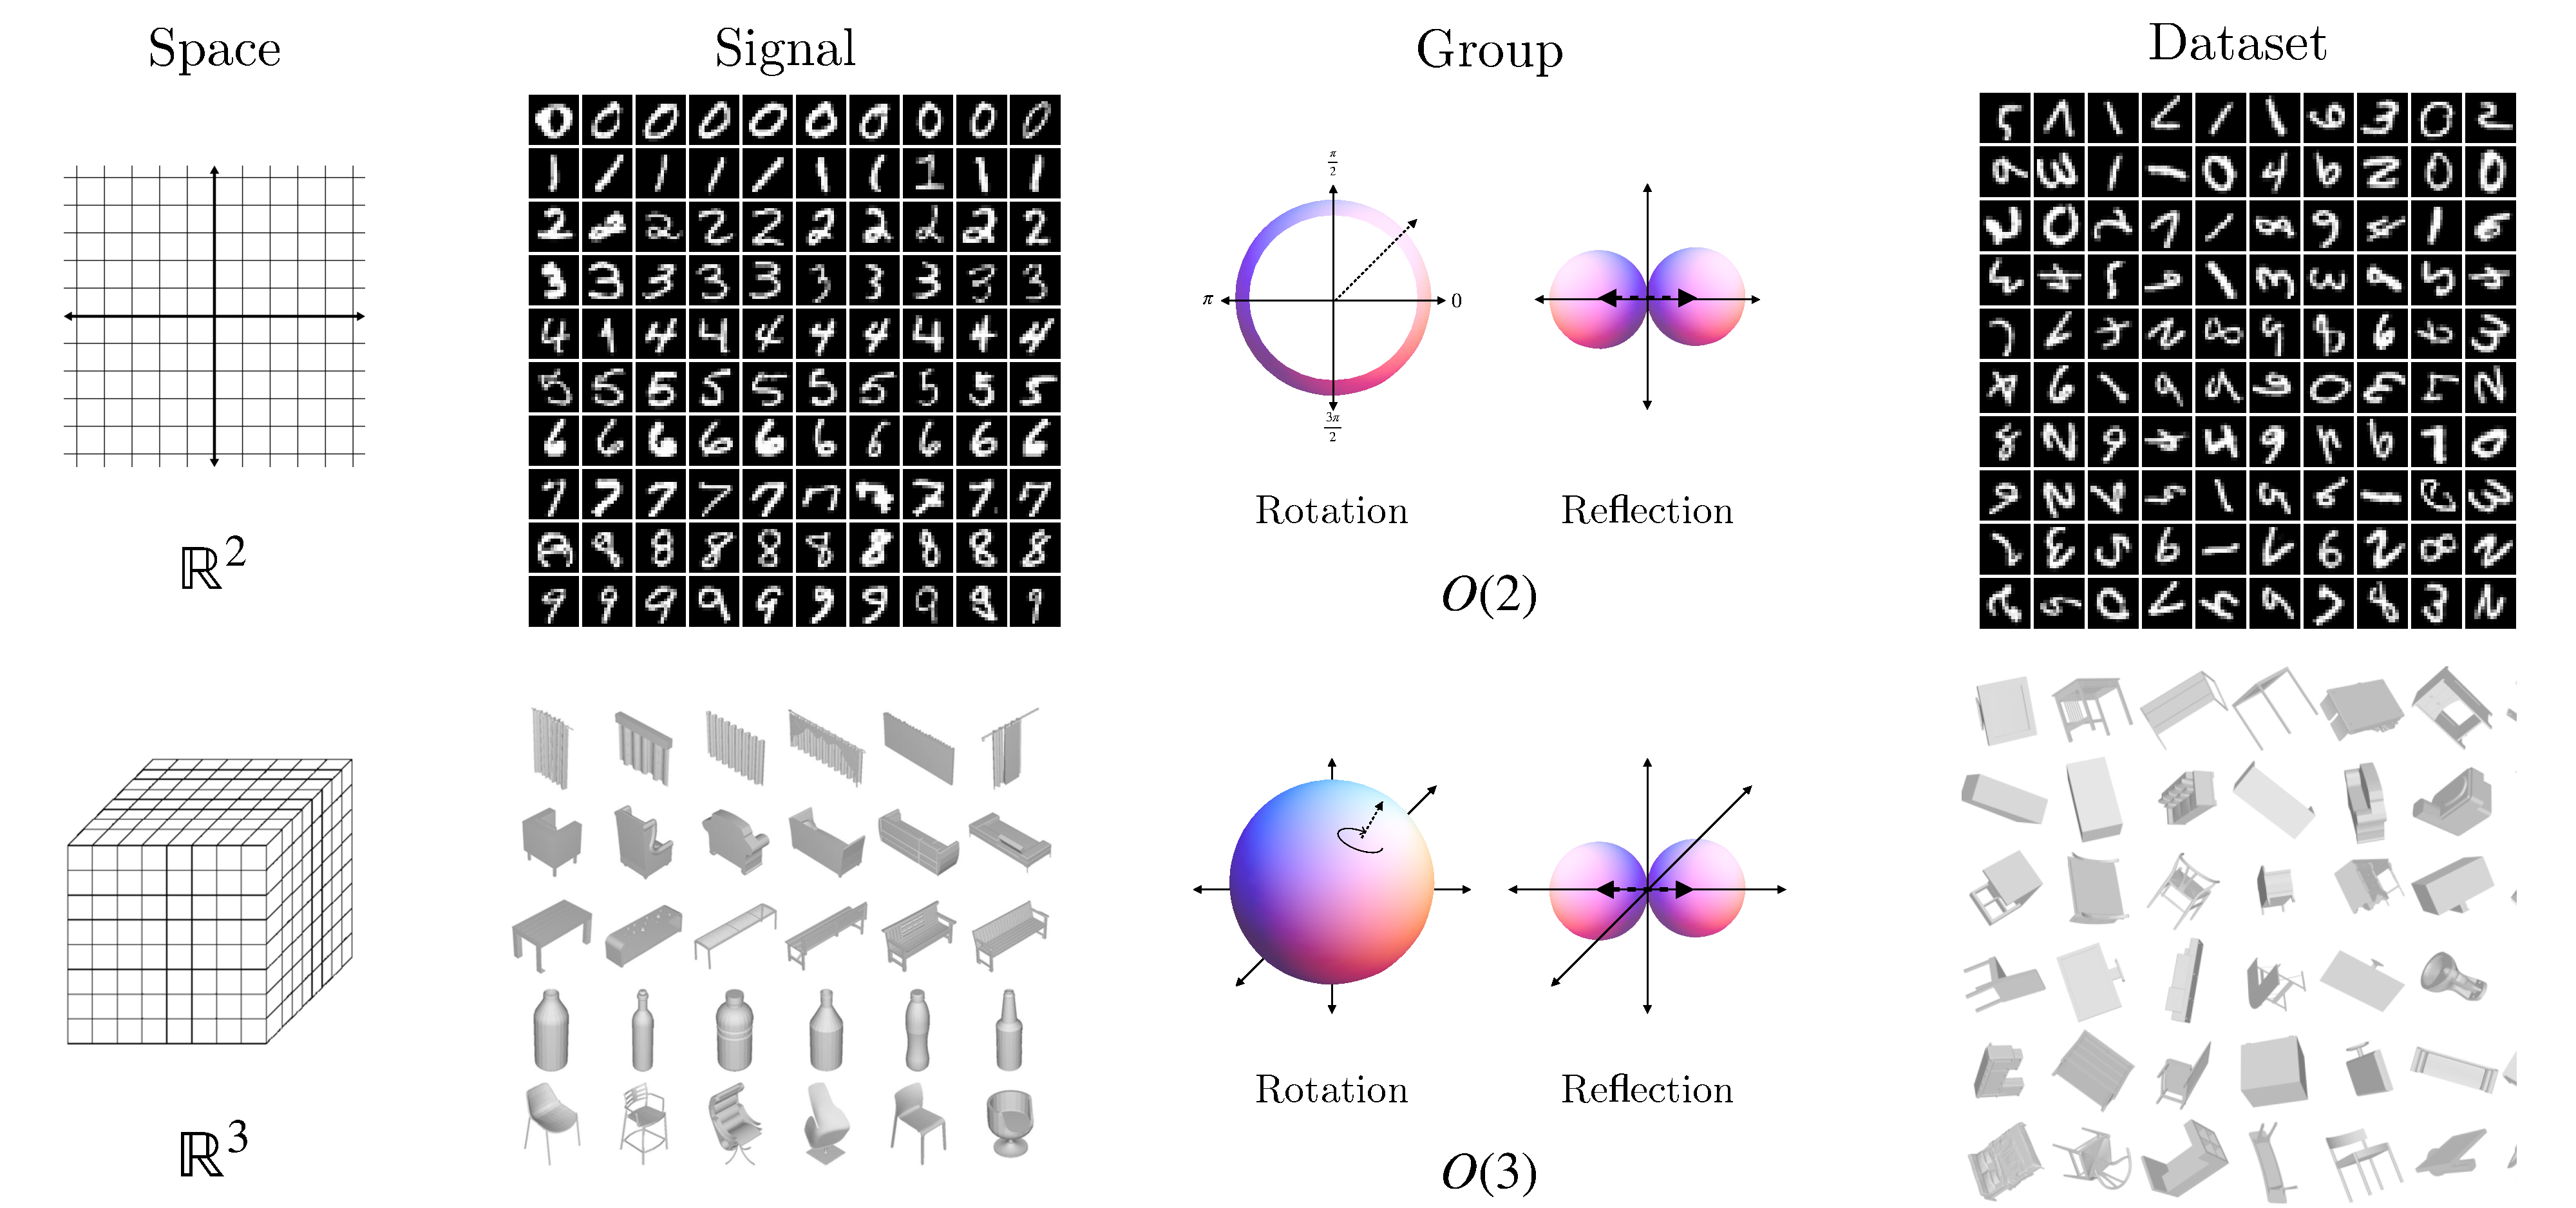
\includegraphics[width=\linewidth]{figs/datasets.pdf}
    \caption{\textbf{Datasets.} The $O(2)$-MNIST (top) and $O(3)$-ModelNet10 (bottom) datasets are generated by applying a random (rotation, reflection) pair to each element of the original datasets. Although we visualize the continuous group here, in practice, we discretize the group $O(3)$ as the full octahedral group $O_h$ to reduce computational complexity. $SO(2)$ and $SO(3)$ datasets are generated similarly, by applying a random rotation to each datapoint.}
    \label{fig:datasets}
\end{figure}

In these experiments, we train pairs of models in parameter-matched architectures, in which only the $G$-Pooling method differs. Note that the purpose of these experiments is to compare \textit{differences in performance} between models using Max $G$-Pooling vs. the $G$-TC\textemdash not to achieve SOTA accuracy. Thus, we do not optimize the models for overall performance. Rather, we fix a simple architecture and set of hyperparameters and examine the change in performance that arises from replacing Max $G$-Pooling with the $G$-TC Layer (Figure \ref{fig:models}).

\begin{figure}[H]
    \centering
    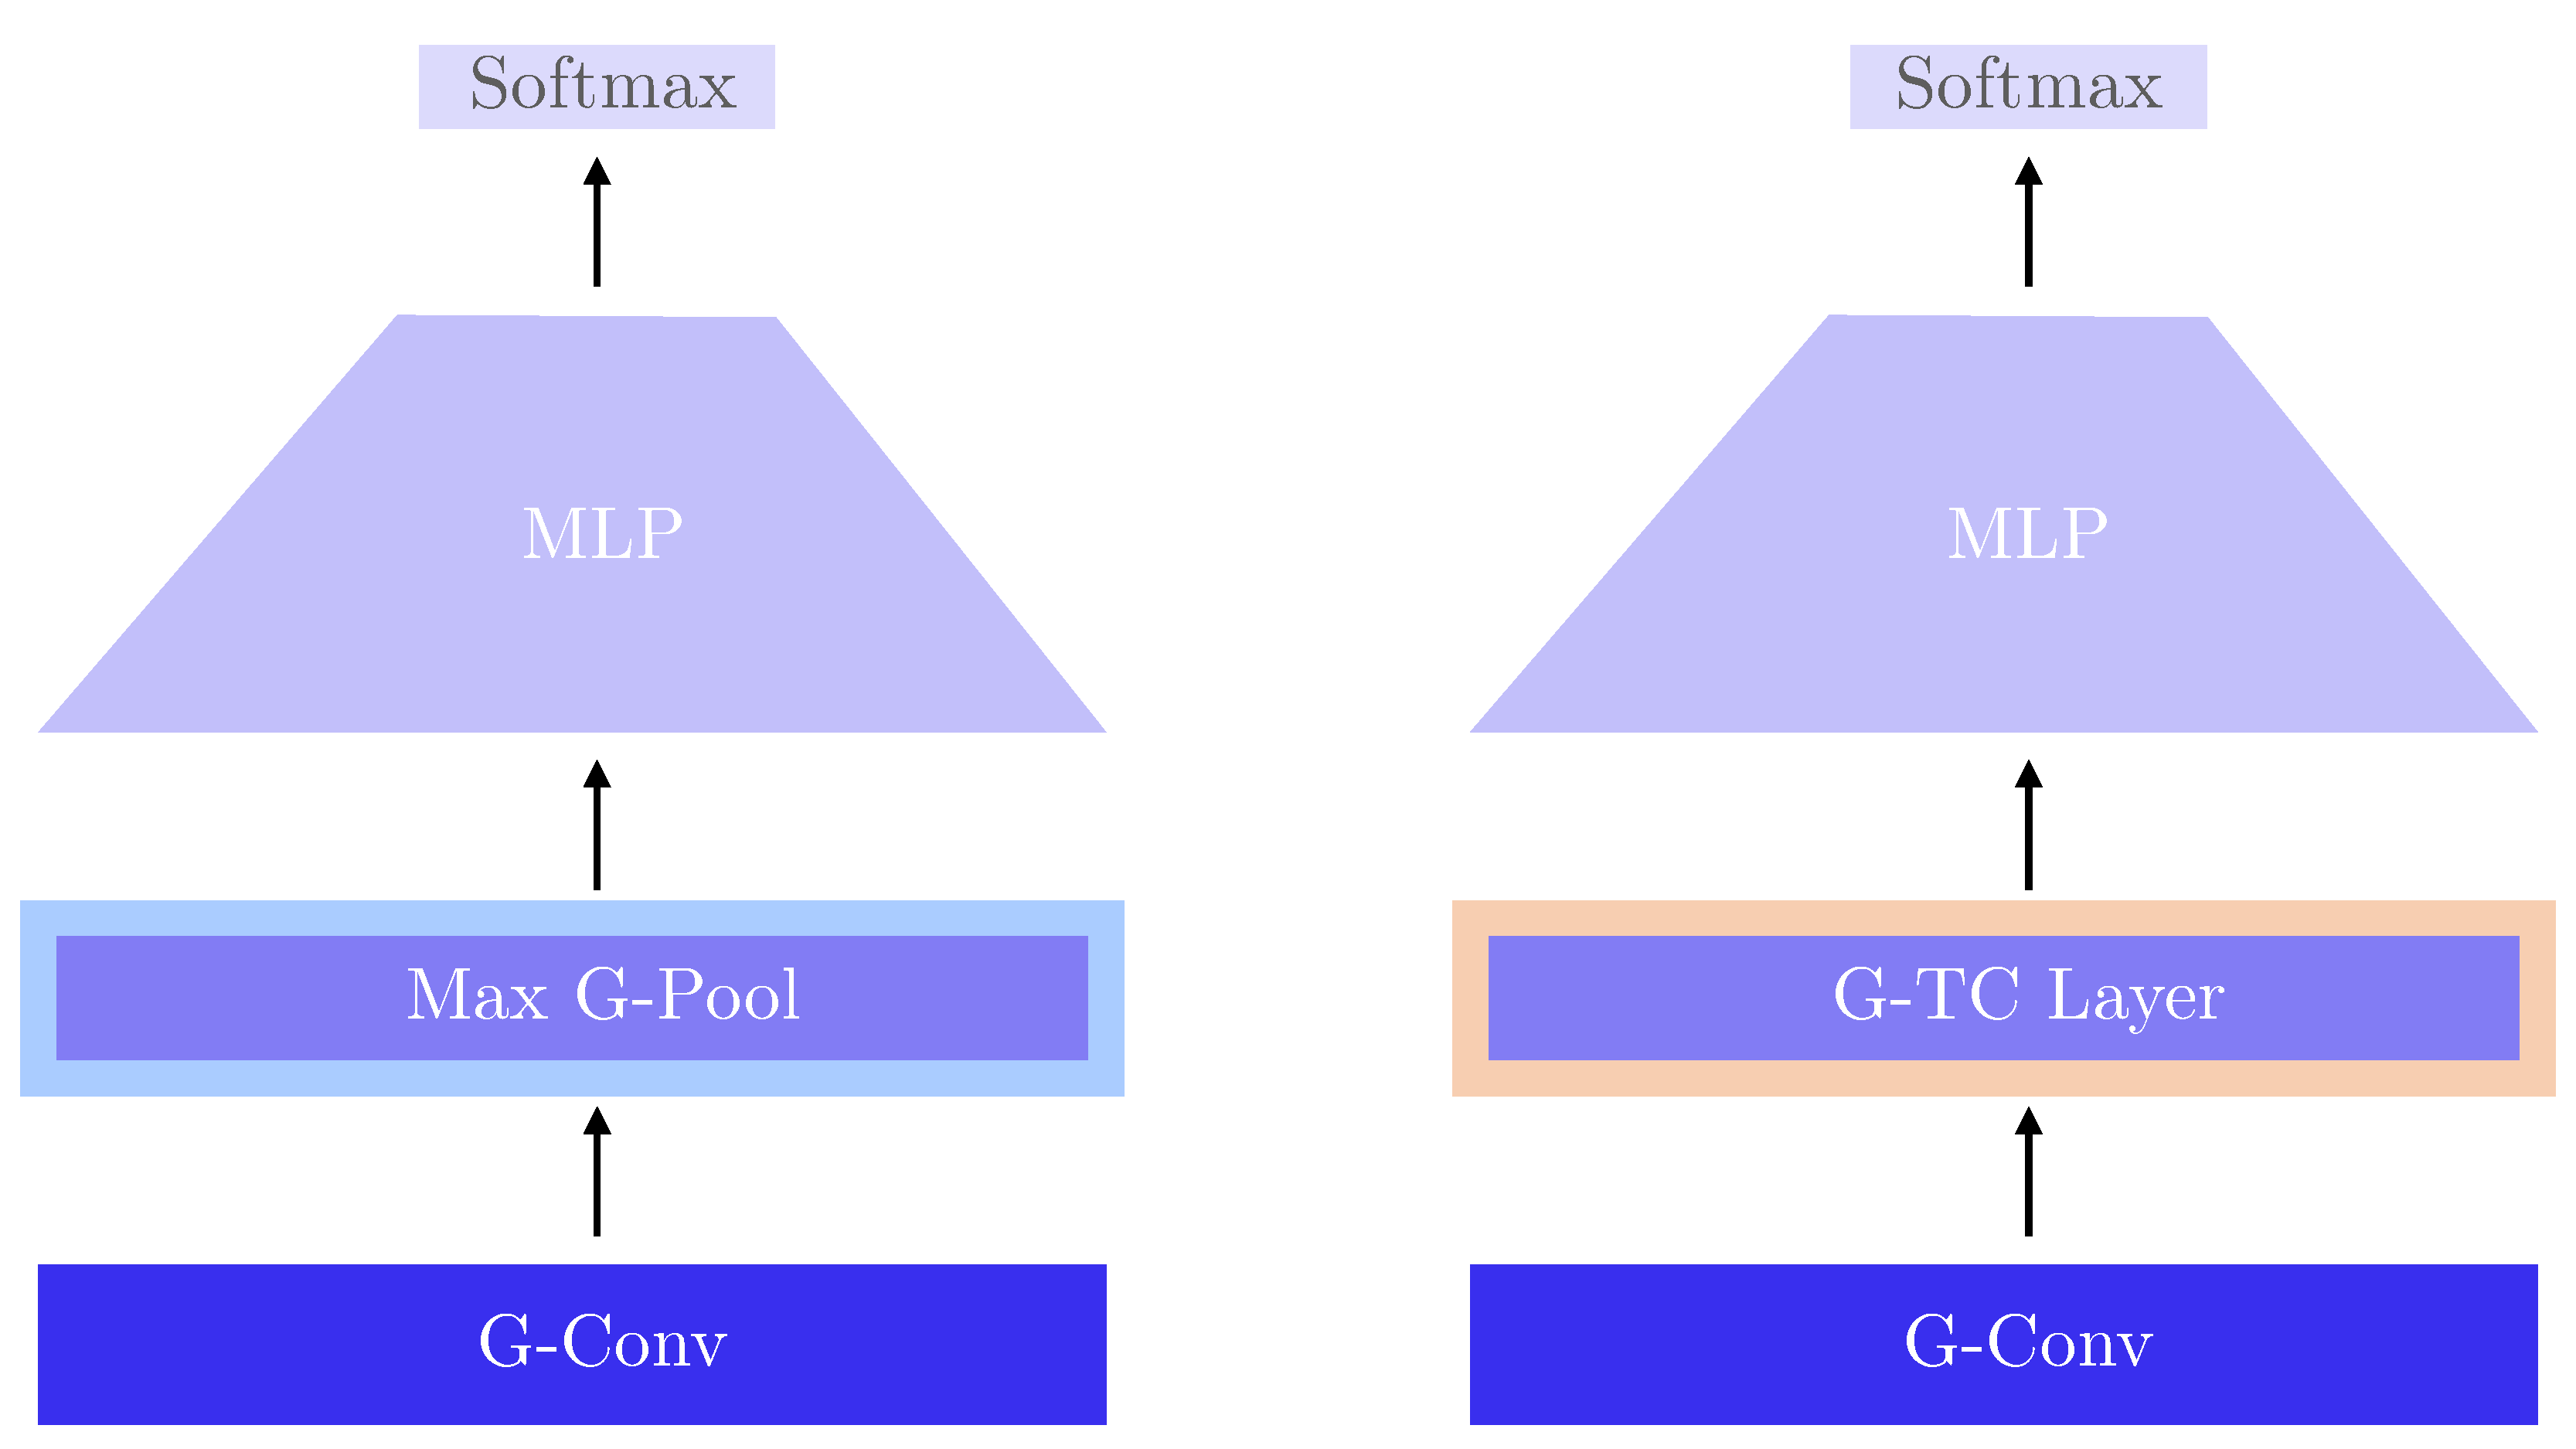
\includegraphics[width=0.5\linewidth]{figs/models.pdf}
    \caption{\textbf{Models.} We compare two simple architectures comprised of a single G-Conv block followed by either a Max $G$-Pool layer or a $G$-TC Layer and an MLP Classifier.}
    \label{fig:models}
\end{figure}

To isolate the effects of the $G$-Pooling method, all models are comprised of a single $G$-Conv block followed by $G$-Pooling (Max or TC) and an MLP Classifier. Notably, while many $G$-Conv models in the literature use the semi-direct product of $G$ with $\mathbb{R}^n$\textemdash i.e. incorporating the actions of the group $G$ into a standard translational convolutional model\textemdash here, we perform only \textit{pure} $G$-Conv, without translation. Thus, we use filters the same size as the input in all models.  The $G$-Conv block is comprised of a $G$-Conv layer, a batch norm layer, and an optional nonlinearity. For the Max $G$-Pool model, ReLU is used as the nonlinearity. Given the third-order nonlinearity of the TC, we omit the nonlinearity in the $G$-Conv block in the TC Model. The $G$-TC layer increases the dimensionality of the output of the $G$-Conv block; consequently the input dimension of the first layer of the MLP is larger and the weight matrix contains more parameters than for the Max $G$-Pool model. To compensate for this, we increase the dimension of the output of the first MLP layer in the Max Model, to match the overall number of parameters.


% and find it to be sufficient to obtain high classification accuracy. Moreover, we find that the ReLU loses information in the $G$-Conv that must be preserved to obtain completeness in the TC Layer.
% For this reason, we rescale the MNIST dataset to $(16, 16)$ pixels and voxelize ModelNet10 with a grid of shape $(10, 10, 10)$.




\subsubsection*{Evaluation Methods}

We evaluate the models in two ways. First, we examine differences in the raw \textit{classification accuracy} obtained by replacing Max $G$-Pooling with the $G$-TC Layer. Second, we assess the \textit{completeness} of the model by optimizing ``metameric'' stimuli for the trained models\textemdash inputs that yield the same pre-classifier representation as a target input, but are perceptually distinct. The completeness evaluation is inspired by a recent paper that incorporates the bispectrum\textemdash the spectral dual of the triple correlation\textemdash into a neural network architecture trained to yield $G$-invariant representations for $G$-transformed data \cite{sanborn2023bispectral}. In this work, two inputs are considered ``perceptually distinct'' if they are not in the same group orbit. They find that all inputs optimized to yield the same representation in the bispectral model are identical up to the group action. By contrast, many metameric stimuli can be found for $E(2)$-CNN \cite{e2cnn}, a $G$-Equivariant CNN that uses Max $G$-Pooling. Given the duality of the bispectrum and the triple correlation, we expect to observe similar ``completeness'' for $G$-CNNs using the $G$-TC Layer.



% For this evaluation, we draw inspiration from a recent paper on a neural network architecture based on the bispectrum, the spectral dual of the triple correlation \cite{sanborn2023bispectral}. The bispectrum, like the triple correlation, is a \textit{complete invariant}. To assess the completeness of the model, the authors optimize ``metameric'' stimuli for their model, as well as


% TC $G$-Pooling layer substitute for the conventional Max $G$-Pooling


% \subsection{MNIST Experiments: $SO(2)$ and $O(2)$ on $\mathbb{R}^2$}

\subsection{Classification Performance}


% Table \ref{tab:mnist} shows the approximately matched parameter counts for each model.

We train $G$-TC and Max $G$-Pooling models on the $SO(2)$ and $O(2)$-MNIST and chiral ($O$) and full ($O_h$) octahedral voxelized ModelNet10 training datasets and examine their classification performance on the test set. Full training details including hyperparameters are provided in Appendix~\ref{app:training}. Table \ref{tab:mnist} shows the test classification accuracy obtained by the Max-$G$ and $G$-TC architectures on each dataset. Accuracy is averaged over four random seeds, with confidence intervals showing standard deviation. We find that the model equipped with $G$-TC obtains a substantial improvement in overall classification performance\textemdash an increase of $1.3$, $0.89$, $1.84$ and $3.49$ percentage points on $SO(2)$-MNIST, $O(2)$-MNIST, $O$-ModelNet10 and $O_h$-ModelNet10 respectively.


\begin{table}[H]
\centering
\begin{tabular}{c cc cc}
\toprule
& \multicolumn{2}{c}{ \textbf{$C8$-CNN on $SO(2)$-MNIST}} & \multicolumn{2}{c}{\textbf{$D16$-CNN on $O(2)$-MNIST}} \\
\cmidrule(lr){2-3} \cmidrule(l){4-5}
Method & Accuracy & Parameters & Accuracy & Parameters \\
\midrule
% \cmidrule(lr){2-3} \cmidrule(l){4-5}
Max $G$-Pool & 95.23 $\pm$ 0.15 & 32,915 & 92.17\% $\pm$ 0.23 & 224,470 \\
\textbf{$G$-TC} & \textbf{96.53} $\pm$ \textbf{0.16}  &  35,218 & \textbf{93.06 \% $\pm$ 0.09} & 221,074 \\
\bottomrule
\end{tabular}

\begin{tabular}{c  cc cc}
\toprule
& \multicolumn{2}{c}{ \textbf{$O$-CNN on $O$-ModelNet10}} & \multicolumn{2}{c}{\textbf{$O_h$-CNN on $O_h$-ModelNet10}} \\
\cmidrule(lr){2-3} \cmidrule(l){4-5}
Method & Accuracy & Parameters & Accuracy & Parameters \\
\midrule
Max $G$-Pool & 72.17\% $\pm$ 0.95 & 500,198 & 71.73\% $\pm$ 0.23  & 1,826,978 \\
% \textbf{$G$-TC} & \textbf{75.29\%} $\pm$ \textbf{0.86} & \textbf{476,354} & \textbf{76.69\%} $\pm$ \textbf{0.72} & \textbf{1,821,890} \\
\textbf{$G$-TC} & \textbf{74.01\%} $\pm$ \textbf{0.48} & \textbf{472,066} & \textbf{75.22\%} $\pm$ \textbf{0.62} & \textbf{1,817,602} \\

\bottomrule \\
\end{tabular}

  \caption{\textbf{Classification Accuracy \& Parameter Counts for Models Trained on $G$-MNIST and $G$-ModelNet10}. Confidence intervals reflect standard deviation over four random seeds per model. The model equipped with $G$-TC rather than Max $G$-Pooling obtains improved classification performance on all datasets.}
\label{tab:mnist}
\end{table}

% \begin{table}[H]
% \centering
% \begin{tabular}{c  cc cc}
% \toprule
% & \multicolumn{2}{c}{ \textbf{$O$-CNN on $O$-ModelNet10}} & \multicolumn{2}{c}{\textbf{$O_h$-CNN on $O_h$-ModelNet10}} \\
% \cmidrule(lr){2-3} \cmidrule(l){4-5}
% Method & Accuracy & Parameters & Accuracy & Parameters \\
% \midrule
% Max $G$-Pool & 72.17\% $\pm$ 0.95 & 500,198 & 71.73\% $\pm$ 0.23  & 1,826,978 \\
% \textbf{TC $G$-Pool} & \textbf{75.29\%} $\pm$ \textbf{0.86} & \textbf{476,354} & \textbf{76.69\%} $\pm$ \textbf{0.72} & \textbf{1,821,890} \\
% \bottomrule
% \end{tabular}
% \vspace{0.2cm}
%   \caption{\textbf{Classification Accuracy \& Parameter Counts for Models Trained on $G$-ModelNet10}.  Confidence intervals reflect standard deviation over five random seeds per model. }
% \label{tab:modelnet}
% \end{table}

% \begin{table}[H]

%   \centering
%   \begin{tabular}{ccc}
%     \toprule
%     \textbf{Pooling Method} & \textbf{$C8$-CNN on $SO(2)$-MNIST} & \textbf{$D16$-CNN on $O(2)$-MNIST}  \\
%     \midrule
%     Max $G$-Pool & Score & 93.58\%  \\
%     \textbf{TC} \textbf{$G$-Pool} & \textbf{Score} & \textbf{97.16\%} \\
%     \bottomrule
%     \\
%   \end{tabular}
%   \caption{\textbf{Classification Performance on Transformed MNIST Datasets}.}
%   \label{tab:mnist-classification}
% \end{table}

% \begin{table}[H]
%   \centering
%   \begin{tabular}{ccc}
%     \toprule
%     \textbf{Pooling Method} & \textbf{$C8$-CNN on $SO(2)$-MNIST} & \textbf{$D16$-CNN on $O(2)$-MNIST}  \\
%     \midrule
%     Max $G$-Pool & Count & Count  \\
%     \textbf{TC} \textbf{$G$-Pool} & Count & Count\\
%     \bottomrule
%     \\
%   \end{tabular}
%   \caption{\textbf{Parameter Count for MNIST Models}}
%   \label{tab:mnist-params}
% \end{table}

% \begin{figure}[H]
%     \centering
%     \includegraphics[width=0.3\textwidth]{example-image-a}
%     \caption{[Figure showing classification performance]}
%     \label{fig:mnist-classification}
% \end{figure}



\subsection{Completeness}
Following the analysis of \cite{sanborn2023bispectral}, we next evaluate the completeness of the models trained on the $G$-MNIST Dataset. Figure \ref{fig:mnist-completeness} shows inputs optimized to yield the same pre-classifier representation as a set of target images. In line with similar findings from \cite{sanborn2023bispectral}, we find that all inputs yielding an identical representations and classifications in the $G$-TC Model are within the same group orbit. Notably, the optimized images are identical to the targets, \textit{up to the group action}. This reflects exactly the completness of the $G$-TC: the $G$-TC preserves all signal structure up to the group action. Thus, any rotated version of the a target will yield the same $G$-TC Layer output. By contrast, many ``metameric'' misclassified stimuli can be found for the Max $G$-Pool Model, a consequence of the lossiness of this pooling operation.


\begin{figure}[h]
    \centering
    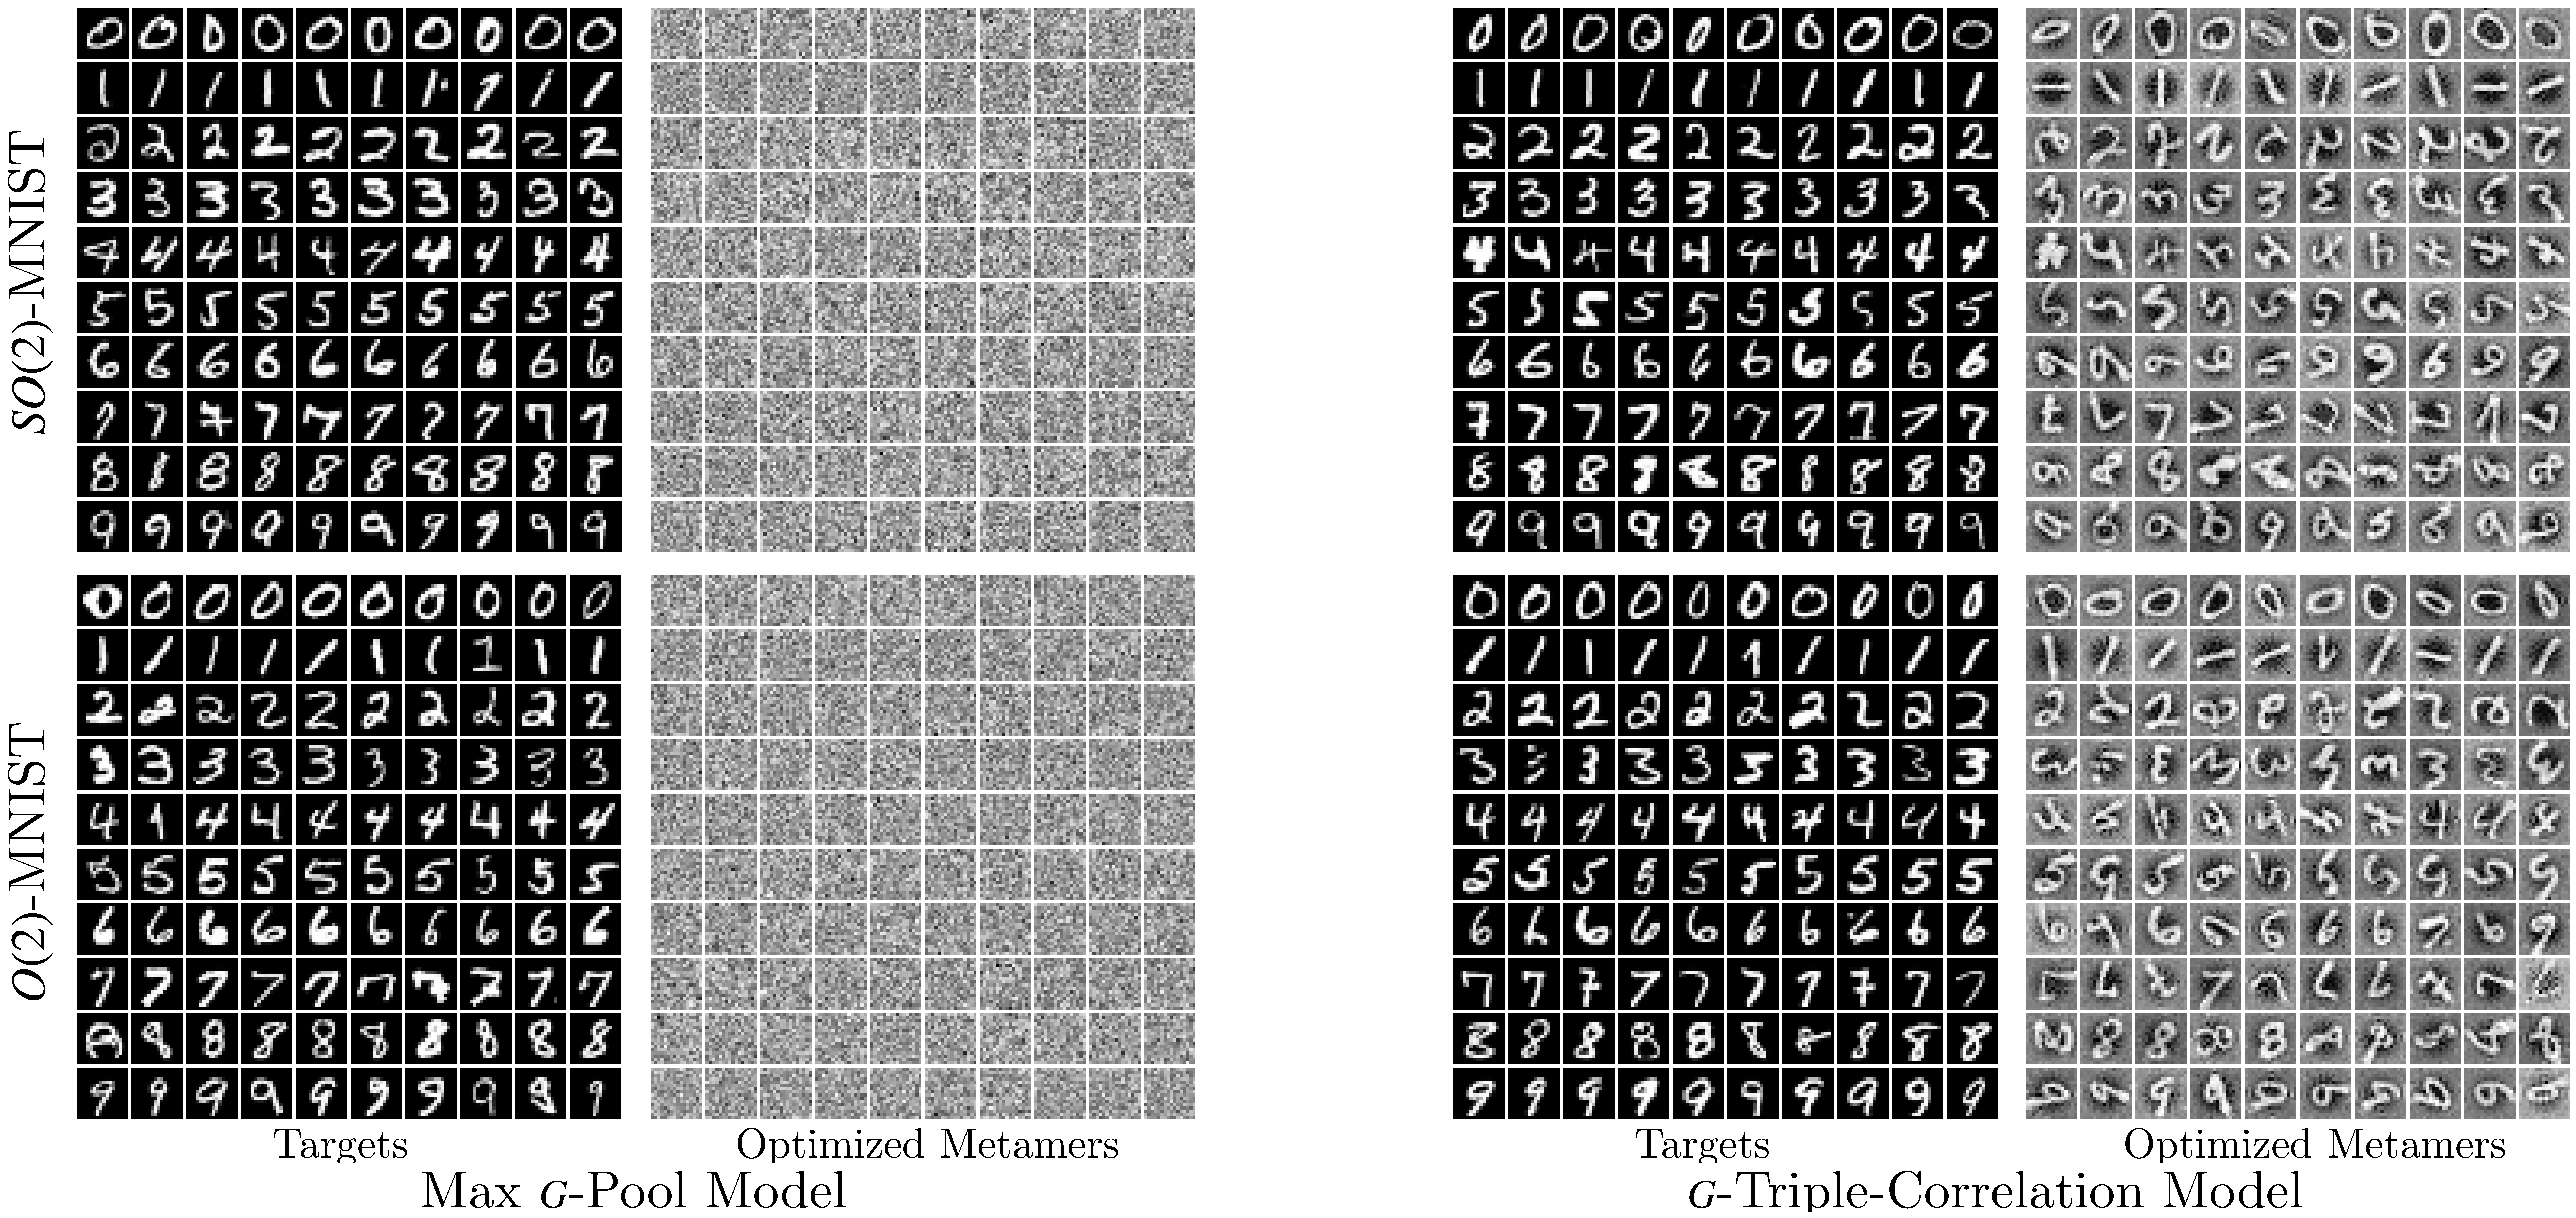
\includegraphics[width=\textwidth]{figs/so2-o2-metamers.pdf}
    % 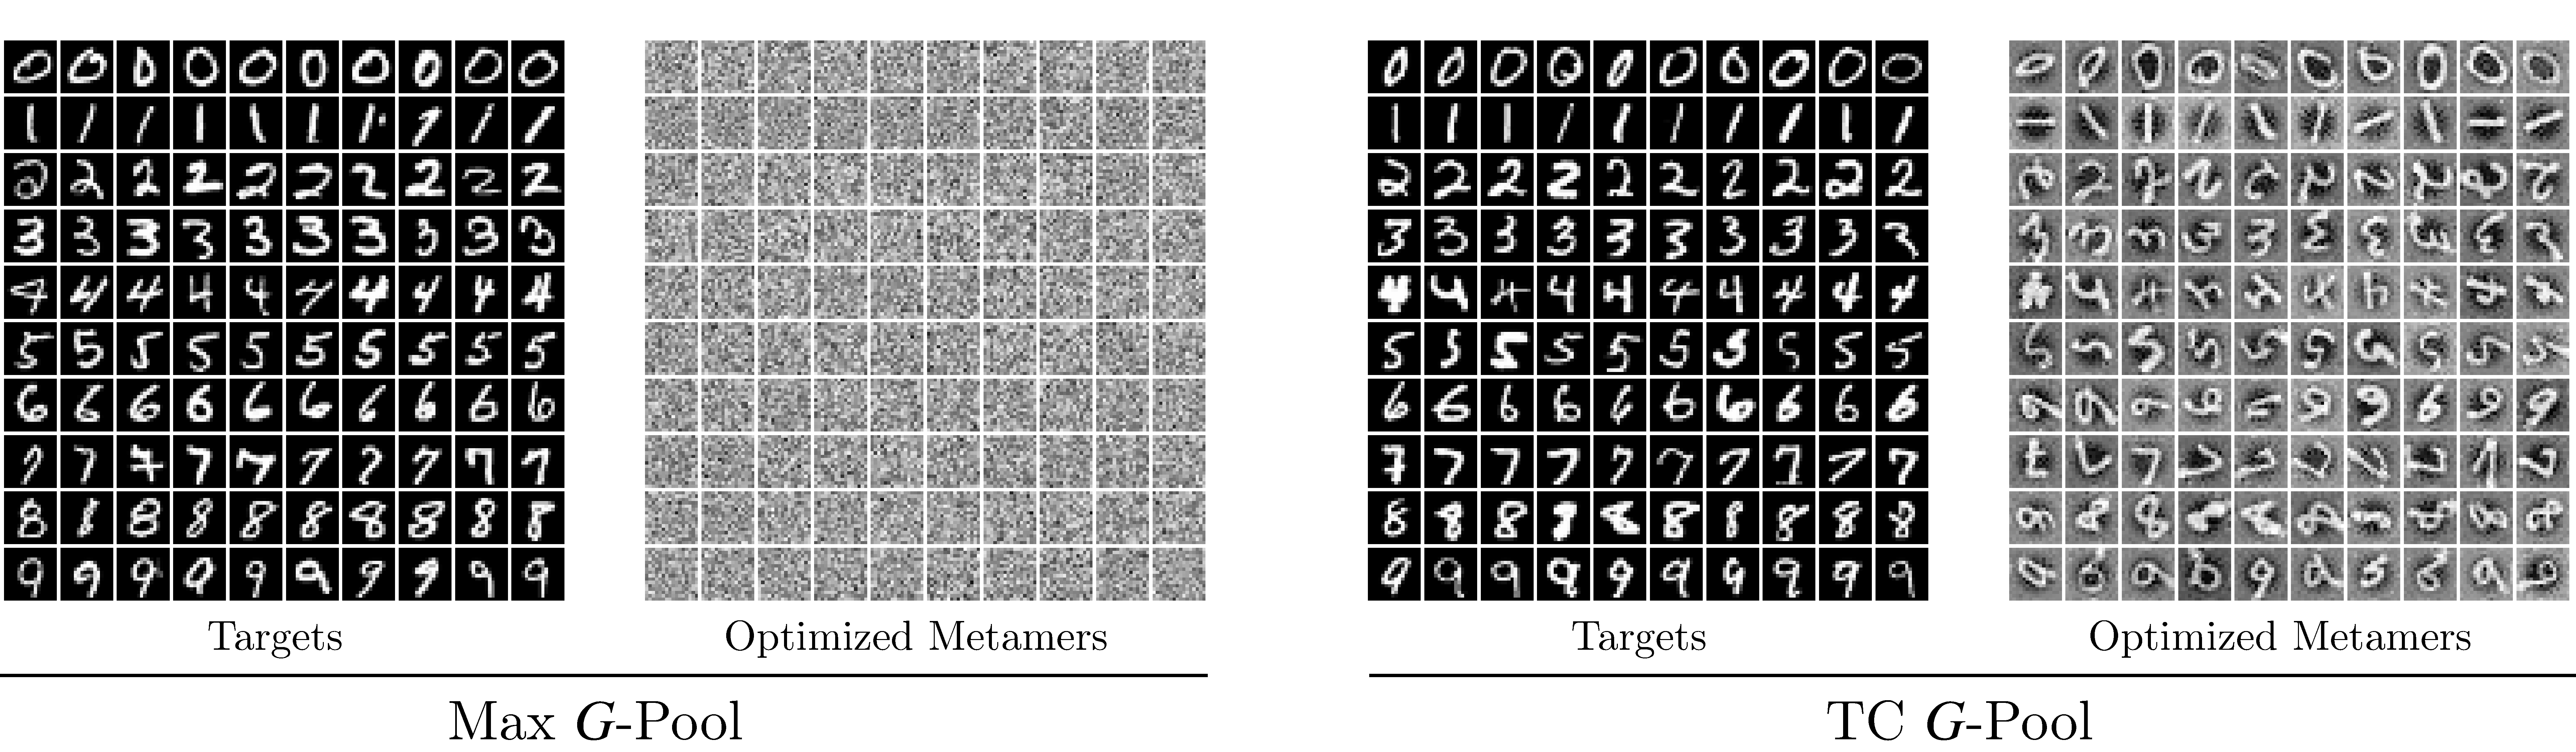
\includegraphics[width=\textwidth]{figs/so2-metamers.pdf}
    % \includegraphics[width=0.3\textwidth]{example-image-b}
    % \includegraphics[width=0.3\textwidth]{example-image-b}
    \caption{\textbf{Optimized Model Metamers.} For each model, 100 targets from the MNIST dataset were randomly selected. 100 inputs were randomly initalized and optimized to yield identical pre-classifier model presentations. All inputs optimized for the $G$-TC Model converge to the orbit of the target. By contrast, metamers that bear no semantic relationship to the targets are found for every target in the Max $G$-Pooling model. \vspace{-0.4cm}}
    \label{fig:mnist-completeness}
\end{figure}

% \subsection{ModelNet10 Experiments: $SO(3)$ and $O(3)$ on $\mathbb{R}^3$}

% \paragraph*{Classification Accuracy.} We next train models on the chiral ($O$) and full ($O_h$) octahedral voxelized ModelNet10 training datasets and examine their classification performance on the test set. Full training details including hyperparameters are provided in the appendix. Table \ref{tab:modelnet} shows the test classification accuracy obtained by the Max and TC architectures on the $O$ and $O_h$ datasets. Accuracy is averaged over six random seeds, with confidence intervals showing standard deviation. As in the previous experiment, we find that the model equipped with TC $G$-Pooling obtains a substantial improvement in overall classification performance\textemdash an increase in $3.12$ and $4.96$ percentage points on $O$-ModelNet10 and $O_h$-ModelNet, respectively.



% \begin{table}[H]
%   \centering
%   \begin{tabular}{ccc}
%     \toprule
%     \textbf{Pooling Method} & \textbf{$O$-CNN on $O$-ModelNet10} & \textbf{$O_h$-CNN on $O_h$-ModelNet10}  \\
%     \midrule
%     Max $G$-Pool & Score & Score  \\
%     \textbf{TC $G$-Pool} & \textbf{Score} & \textbf{Score} \\
%     \bottomrule
%     \\
%   \end{tabular}
%   \caption{\textbf{Classification Performance on Transformed ModelNet10 Datasets}. Accuracy on the test set is averaged over six random seeds, with confidence intervals showing standard deviation.}
%   \label{tab:simple-table}
% \end{table}


% \begin{table}[H]
%   \centering
%   \begin{tabular}{ccc}
%     \toprule
%     \textbf{Pooling Method} & \textbf{$O$-CNN on $O$-ModelNet10} & \textbf{$O_h$-CNN on $O_h$-ModelNet10}  \\
%     \midrule
%     Max $G$-Pool & Score & Score  \\
%     \textbf{TC $G$-Pool} & \textbf{Score} & \textbf{Score} \\
%     \bottomrule
%     \\
%   \end{tabular}
%   \caption{\textbf{Parameter Count for ModelNet10 Models}}
%   \label{tab:simple-table}
% \end{table}


% \begin{table}[htbp]
%   \centering
%   \begin{minipage}[t]{0.45\linewidth}
%     \centering
%     \caption{Table 1}
%     \begin{tabular}{cc}
%         \toprule
%         \textbf{Pooling Method} & \textbf{$O$-ModelNet10}  \\
%         \midrule
%         Max $G$-Pool & Score \\
%         TC $G$-Pool & Score \\
%         \bottomrule
%     \end{tabular}
%   \end{minipage}
%   \hfill
%   \begin{minipage}[t]{0.45\linewidth}
%     \centering
%     \caption{Table 2}
%     \begin{tabular}{cc}
%     \toprule
%     \textbf{Pooling Method} & \textbf{$O_h$-ModelNet10}  \\
%     \midrule
%     Max $G$-Pool & Score \\
%     TC $G$-Pool & Score \\
%     \bottomrule
%     \end{tabular}
%   \end{minipage}
% \end{table}




% \begin{figure}[H]
%     \centering
%     \includegraphics[width=0.3\textwidth]{example-image-a}
%     \caption{[Figure showing classification performance]}
%     \label{fig:modelnet-classification}
% \end{figure}


% \paragraph{Completeness.} We next evaluate the completeness of the trained models. Figure \ref{fig:modelnet-completeness} shows inputs optimized to yield the same pre-classifier representation as a set of target images. As with the MNIST experiments, we find that all inputs yielding an identical representations in the TC $G$-Pool model are within the same group orbit, while many ``metameric'' stimuli can be found for the Max $G$-Pool model.

% \begin{figure}[H]
%     \centering
%     \includegraphics[width=0.3\textwidth]{example-image-b}
%     \includegraphics[width=0.3\textwidth]{example-image-b} \\
%     % \includegraphics[width=0.3\textwidth]{example-image-b}
%     % \includegraphics[width=0.3\textwidth]{example-image-b}
%     \caption{[Figure showing adversarial examples]}
%     \label{fig:modelnet-completeness}
% \end{figure}


% Compare to this paper: https://arxiv.org/pdf/1911.08251.pdf
